\subsection{Model Environment}

I develop a model of university admissions with students with heterogeneous preference and admission grades and universities with heterogeneous educational quality. The model builds on Epple et al 2006. First, universities face capacity constraints and must set admission thresholds to manage enrollment. Second, students from different types of schools (public and private) compete for admission through their grades. There are two grading schemes: standardized exams and non-standardized exams. The non-standardized exams are not centrally regulated and grades are assigned based on the student's school, demographic attributes, and subject content. Standardized exams assign grades to students without considering the student's attributes and responding to the student's academic ability. Universities adjust thresholds to match the number of admitted students with their capacity. 

I define how grades are assigned to students differently by exam formats. I define a multivariate function \( F \) that maps the ability and attributes of a student, along with the grading scheme, to a distribution of grades. Formally, let
\[
F: \mathbb{R} \times \mathbb{R}^n \times \{ \text{standardized}, \text{non-standardized} \} \to \mathcal{P}(\{\text{A*}, \text{A}, \text{B}, \ldots\}),
\]
where \( e \in \mathbb{R} \) represents the student's actual ability, \( X \in \mathbb{R}^n \) denotes additional student attributes, and \( \mathcal{P}(\{\text{A*}, \text{A}, \text{B}, \ldots\}) \) represents the set of probability distributions over the ordered grade set.

The grade distribution follows:
\[
F(e, X, Y) \sim \mathcal{M}(\vec{p}(e, X, Y)),
\]
where \( \mathcal{M} \) denotes a multinomial distribution and \( \vec{p}(e, X, Y) \) is a vector of probabilities for each grade, respecting the ordinality of grades from A* to lower grades. The vector \( \vec{p} \) is specified based on whether the grading is standardized or non-standardized:
\[
\vec{p}(e, X, Y) =
\begin{cases}
\vec{p}_s(e), & \text{if } Y = \text{standardized}, \\
\vec{p}_{ns}(e, X), & \text{if } Y = \text{non-standardized}.
\end{cases}
\]
For standardized grading, \( \vec{p}_s(e) \) depends only on the ability of the student \( e \), making the classification process objective. However, under non-standardized grading, \( \vec{p}_{ns}(e, X) \) is influenced by both the ability \( e \) and the additional attributes of the student \( X \), introducing a degree of subjectivity based on contextual factors due to reliance on school context and demographic attributes.

\subsection{Universities and Students}
\subsubsection{Students}
% Students
A continuum of students with total mass \(N\) populates the market. Each student \( i \) is characterized by their demographics \( x_i \in \mathcal{R}^n \), attending school type \( s_i \in \{private, public\} \), academic ability score \( e_i^\prime \) and preferences for universities. Note that the observed academic ability score \( e_i^\prime \) is drawn from the grade distribution \(F(e,X,Y)\), where the latent ability \(e\) is transformed by the scoring mechanism based both on the attributes of the student \(X\) and the type of exam
\(Y\).

Students apply to the best university that they meet the university's grade requirements. Students have the following utility function.
\begin{equation*}
    U_{i,j}(e^\prime) = \beta Q_j -p_j
\end{equation*}
\(Q_j\) denotes the quality of university \(j\) and \(\beta\) is its scale parameter. \(p_j\) denotes the tuition that the student must pay. 

Students choose the best school out of all available universities with thresholds lower than their grade. The set of appliable universities is summarized as the following.
\begin{equation*}
    \mathcal{J}^\prime(e^\prime) \equiv \{j\in \mathcal{J}| e_j^*\leq e^\prime\}
\end{equation*}
\(e_j^*\) denotes the equilibrium grade threshold that university \(j\) sets.

I assume tuition is uniform across universities. 

The best response of students simplifies to applying to the highest quality school that their grade permit.

\subsubsection{Universities}
Universities maximize profits given tuition and their capacity to accommodate students. Universities pay a penalty term for any discrepancy between their capacity and the volume of incoming students. I define a university's profit function as the following.
\begin{equation*}
    \pi_j = p\int_{s^*}^{s^{**}}dF -\gamma_j \left(\int_{s^*}^{s^{**}}dF-k_j \right) ^2
\end{equation*}
\(k\) denotes the capacity of university \(j\), and \(s_j^*\) denotes the threshold score of the university and \(s_j^{**}\) denotes the threshold of the university that set a threshold above them. 

The best response of the universities is the following.
\begin{equation*}
    s_j^* = F^{-1}\left((F(s_j^{**})-k)-\frac{p}{2\gamma_j}\right)
\end{equation*}

\subsection{Definition of Equilibrium}

\begin{definition}[Student Best Response]
A student with grade $e'$ attends university
\[
j^*(e') = \arg\max_{j \in \mathcal{J}'(e') \cup \{0\}} \{ \beta Q_j - p \},
\]
with the outside option normalized to $0$.
\end{definition}

\begin{definition}[University Best Response]
University $j$ chooses a grade threshold $e_j^*$ that maximizes its profit:
\[
e_j^* \in \arg\max_{e\in [e_{\min}, e_{\max}]} \left\{ p \int_{e' \ge e} dF(e') - \gamma_j \Bigl(\int_{e' \ge e} dF(e') - k_j\Bigr)^2 \right\}.
\]
\end{definition}

\begin{definition}[Market Equilibrium]
A market equilibrium consists of a quality function Q($\cdot$); a set of universities \{1,2,3,..., J\}; a vector of capacities ($K_1, ..., K_J$): admission thresholds ($\Bar{c}_1, ..., \Bar{c}_J$); a cost function $C$: a continuous distribution $F$ of students: and a grading function G().

A competitive equilibrium for this economy consists of admission thresholds function C(F), and an allocation of students into the $J$ colleges and no college such that;
\begin{enumerate}
    \item For every university $j$, $e_j^*$ maximizes the profit function $\pi_j(e, K)$.
    \item Given the thresholds $\{e_j^*\}$, each student with grade $e'$ attends
    \[
    j^*(e') = \arg\max_{j \in \mathcal{J}'(e') \cup \{0\}} \{ \beta Q_j - p \},
    \]
    provided $\beta Q_j - p>0$.
    \item The resulting allocation of students is consistent with the universities' profit-maximizing decisions.
\end{enumerate}
\end{definition}

\subsection{Proof of Existence of Equilibrium}

\begin{theorem}[Existence of Equilibrium]
An equilibrium in the above admissions market exists.
\end{theorem}

\begin{proof}
We outline the proof in several steps:
\begin{enumerate}
    \item \textbf{University Optimization:} For each university $j$, consider the profit function
    \[
    \pi_j(e) = p \cdot \mu_j(e) - \gamma_j\Bigl(\mu_j(e)-k_j\Bigr)^2,
    \]
    where $\mu_j(e)=\int_{e' \ge e} dF(e')$. Since $F$ is continuous and strictly increasing, $\mu_j(e)$ is continuous and strictly decreasing in $e$. The function $\pi_j(e)$ is continuous on the compact set $[e_{\min}, e_{\max}]$, so by the Extreme Value Theorem, there exists an $e_j^*$ that maximizes $\pi_j(e)$.

    \item \textbf{Student Best Response:} Given the thresholds $\{e_j^*\}$, every student with grade $e'$ is admitted to all universities with $e' \ge e_j^*$. Because all students face the same tuition and their utility is $U_j(e')=\beta Q_j-p$, the best response for any student is to attend the highest quality university among those for which $e'\ge e_j^*$. This decision rule is unique and deterministic.

    \item \textbf{Consistency and Fixed-Point:} The university decision (choosing $e_j^*$ to maximize $\pi_j$) and the student best response (attending the best available university) are interdependent only through the thresholds $\{e_j^*\}$. Define a mapping $\Phi: [e_{\min}, e_{\max}]^J \to [e_{\min}, e_{\max}]^J$ by
    \[
    \Phi_j(\{e_k\}) = \arg\max_{e\in [e_{\min}, e_{\max}]} \left\{ p \int_{e' \ge e} dF(e') - \gamma_j\left(\int_{e' \ge e} dF(e') - k_j\right)^2 \right\}.
    \]
    This mapping is continuous and maps a compact, convex set into itself. By Brouwer's Fixed Point Theorem, there exists a fixed point $\{e_j^*\}$ such that $\Phi_j(\{e_k^*\}) = e_j^*$ for all $j$. At this fixed point, the thresholds and the induced student allocation constitute an equilibrium.
\end{enumerate}
Thus, an equilibrium exists.
\end{proof}

\subsection{Properties of Equilibrium: Sorting}

\begin{proposition}[Sorting Property]
In equilibrium, higher-quality universities admit only students with higher grades. In particular, if $Q_i > Q_j$, then the equilibrium thresholds satisfy $e_i^* > e_j^*$, ensuring that students with higher ability (and hence higher $e'$) attend higher-quality universities.
\end{proposition}

\begin{proof}
\end{proof}

\subsection{Simulation Results}
Simulation results indicate that the share of private school educated students increases with non-standardized exams. I set parameter values as the following.
\begin{tcolorbox}
\begin{itemize}
    \item F is a normal distribution: \(N(\mu_j, \sigma_j)\).

    Standardized: $\mu = 0.0$
    $\sigma = 1.0$

    Non-Standardized: $\mu_{public} = 0.0$.
    $\sigma_{public} = 1.0$.
    $\mu_{private} = 0.5$.
    $\sigma_{private} = 1.2$.
    
    \item \(\gamma_j = 150, \forall j\)
    \item 40\% of students are privately educated.
\end{itemize}
\end{tcolorbox}
\begin{figure}
    \centering
    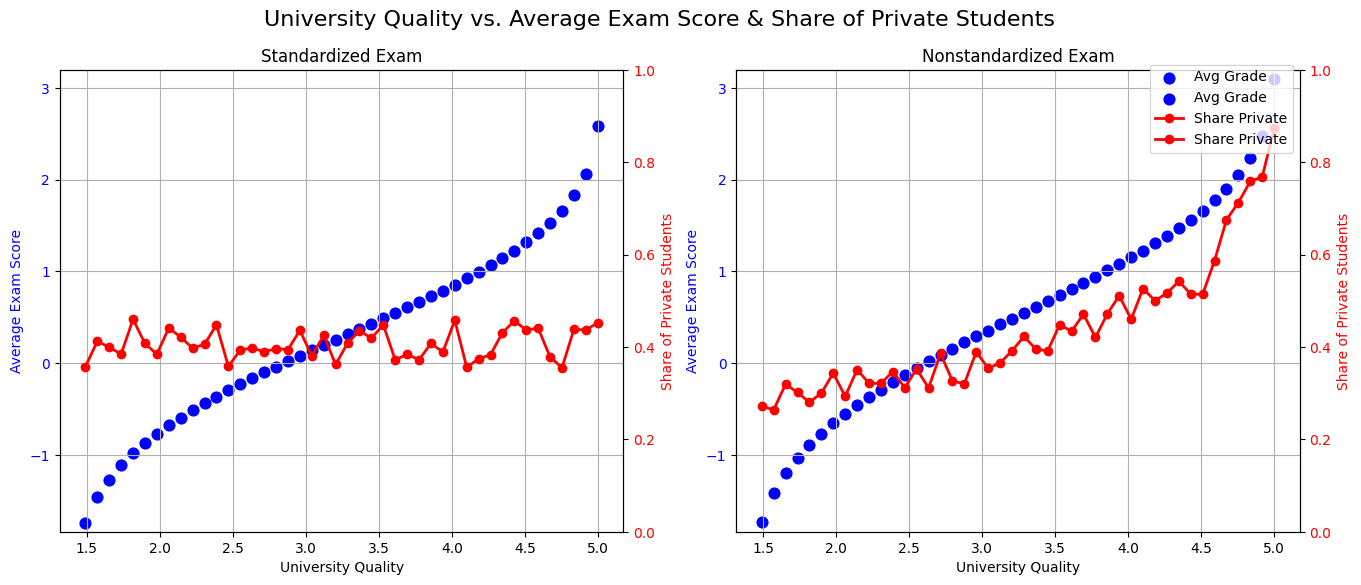
\includegraphics[width = \linewidth]{figures/Empirical_Model/SimulationResult.png}
    \label{fig:enter-label}
\end{figure}

\subsection{Identification}
I discuss how to identify the parameters associated with the cost function. I estimate $\{K_j, C_j\}_{j=1}^J$ for a large sample of universities of size $J$. I assume that universities marginal cost with accepting students is specified as the following.
\begin{equation*}
    C_j = f(|K_j-N_j|) = \alpha + \gamma_j(K_j-N_j) + \epsilon 
\end{equation*}
I estimate $\gamma$ by regressing the increments in admission thresholds on the degree of discrepancy between university capacity and cohort size in 2020. I recover the vector of marginal costs estimates for each universities $\{\hat{\gamma_1},..., \hat{\gamma}_J\}$ by the responses of each programs in the university.

I assume that the students are heterogeneous with respect to their demographics, 

\subsection{Calibration}
Using the estimated distribution of grades and university marginal cost estimates, my model predicts the composition of students at each university. 

To avoid modeling the application behavior of students, I constraint the option set of universities that a student can choose using application portfolio of the 2020 year cohort. 

The alternating grade scheme predicts a grade for 